\documentclass[prb,reprint,amsmath,amssymb,superscriptaddress,floatfix]{revtex4-2}
\usepackage{graphicx}
\usepackage{bm}
\usepackage{dcolumn}
\usepackage[colorlinks=true,linkcolor=blue,citecolor=blue,urlcolor=blue]{hyperref}
\graphicspath{{figures/}}

\newcommand{\ueff}{u_{\rm eff}}
\newcommand{\vm}{\mathbf m}
\newcommand{\vu}{\mathbf u}
\newcommand{\vv}{\mathbf v}
\newcommand{\wone}{\mathbf w_1}
\newcommand{\wtwo}{\mathbf w_2}
\newcommand{\Wtwo}{\mathbf W_2}
\newcommand{\kP}{\kappa_P}
\newcommand{\kt}{\kappa_\tau}
\newcommand{\Dm}{\mathcal D}
\newcommand{\Pg}{\mathcal P}

\begin{document}

\title{Nonreciprocal spin couplings and the Doppler breakdown of driven chiral patterns}

\author{Changyeon Won}
\email{cywon@khu.ac.kr}
\affiliation{Department of Physics, Kyung Hee University, Seoul, Republic of Korea}

\date{\today}

\begin{abstract}
An electric current, or any designed nonreciprocal coupling with a fixed direction, enters the stationary equation of a co-moving chiral magnetic pattern only through two vectors of opposite time-reversal parity, and in Landau--Lifshitz form its dissipative part is exactly $(\beta-\alpha)\vu$, independent of the Hall motion of the pattern.
The residual magnetic group of this structure fixes the first-order response: a helix acquires a cone magnetization $M=s\ueff/D$, a pattern-mediated Edelstein effect, and a skyrmion lattice a dipolar distortion perpendicular to the reactive vector rather than to the current.
A driven pattern has no precessional Walker breakdown, because the restoring force of its conjugate variable does not saturate; its static branch ends instead in a Landau instability of its own Goldstone mode, $\omega_0(k)<\lambda\ueff k$, in which the nonadiabatic parameter enters only through $\ueff=(\beta/\alpha-1)u$.
The order of the Goldstone dispersion decides the threshold, which is finite for a helix, $u_L=D/\sqrt2 s$, and vanishes as $1/L$ for skyrmion lattices and for stripes driven at any angle to their wave vector.
The Doppler efficiency $\lambda$ is a static property of the pattern, one minus the counterflow momentum carried by strain-induced spin canting, and falls from 1 for continuous phase textures to $0.77$--$0.11$ for skyrmion lattices of increasing field; below threshold the same efficiency puts the lattice phonons in a moving Gibbs ensemble, and exchange-even couplings such as damping-like spin--orbit torque pump them through the dual mechanism.
We thus show that the fate of a current-driven chiral pattern is set by the order of its Goldstone dispersion and by a single static number, the Doppler efficiency of its internal relaxation.
\end{abstract}

\maketitle

%======================================================================
\section{Introduction}
\label{sec:intro}

Chiral magnets form spontaneous patterns---helices, stripes and skyrmion lattices---whose period is set by the competition of exchange and the Dzyaloshinskii--Moriya interaction (DMI)~\cite{Muhlbauer2009,Nagaosa2013}. An electric current moves these patterns through the spin-transfer torques of Zhang and Li~\cite{ZhangLi2004,Thiaville2005}, at current densities far below those needed for domain walls~\cite{Jonietz2010,Iwasaki2013}, and Fig.~\ref{fig:patterns} shows the three patterns studied here together with the first effect of a current on each. Two questions about this driven motion remain open. First, a current is a vector with a fixed direction, so it lowers the symmetry of the pattern; which distortions does it then allow, and which does it forbid? Second, a domain wall driven too hard undergoes Walker breakdown~\cite{SchryerWalker1974}; what is the corresponding end of a driven pattern, and what sets its threshold?

Partial answers exist for special cases. A longitudinal current destabilizes a skyrmion string by the emission of Goldstone spin waves once $\omega(k_z)<(\beta/\alpha-1)v_s k_z$~\cite{Okumura2023}, and a current perpendicular to the wave vector of a helix destabilizes it transversely~\cite{Masell2020}. A uniform current exerts no torque on a sixfold skyrmion lattice~\cite{Everschor2012}, and the cone induced in a helix reverses with its chirality~\cite{Jiang2020}. These results use different models and different language. They leave open whether a current can destabilize the in-plane phonons of a skyrmion lattice at all; the string criterion assumes a phase that advances continuously, while a rigid-particle (Thiele) picture of the lattice gives no instability.

Here we treat the current as what it is on a lattice: the antisymmetric part of a nearest-neighbour nonreciprocal spin coupling, $J_{ij}\neq J_{ji}$, with a fixed direction~\cite{Fruchart2021}. In the frame co-moving with a pattern, such a fixed bias enters the stationary equation only through two vectors of opposite time-reversal parity (Sec.~\ref{sec:comoving}). This one structure gives three results. The residual magnetic group fixes the first-order response, with nonsymmorphic protection of the forbidden components (Sec.~\ref{sec:groups}). A pattern has no precessional Walker breakdown; its static branch ends in a Landau instability of its own Goldstone mode, whose threshold is finite or zero according to the order of the dispersion (Secs.~\ref{sec:walker} and \ref{sec:tests}). And the strength of the coupling between the current and that mode is a static property of the pattern, the Doppler efficiency $\lambda$, set by the counterflow of strain-induced spin canting (Sec.~\ref{sec:lambda}). Below threshold the same $\lambda$ defines a moving Gibbs ensemble of the lattice phonons (Sec.~\ref{sec:gibbs}), and couplings that a current cannot produce, such as nonreciprocal DMI, enter the same framework through a dual mechanism (Sec.~\ref{sec:sot}). Section~\ref{sec:real} states where the model's assumptions hold in real samples and lists the predictions as dependencies. What a pattern does beyond its threshold is the subject of a companion paper~\cite{B2}.

\begin{figure}[t]
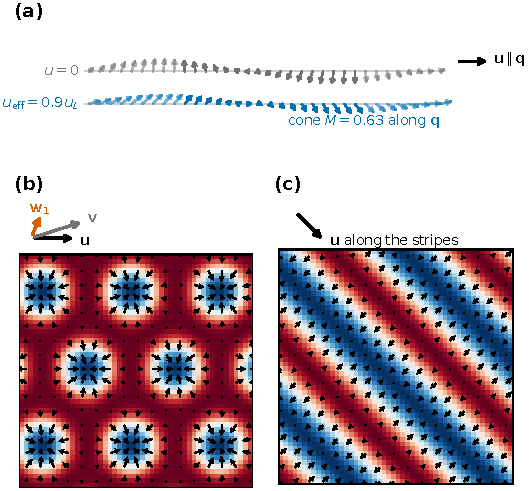
\includegraphics[width=\columnwidth]{figP1_patterns.pdf}
\caption{\label{fig:patterns}The three driven chiral patterns and the first-order effect of a current on each. (a) Bloch helix (every second spin of one period, oblique view): unbiased, and at $\ueff=0.9\,u_L$, where the spins tilt into a cone $M=s\ueff/D$ along $\mathbf q$ [Eq.~(\ref{eq:cone})]. (b) N\'eel skyrmion lattice at $B=0.5D^2/J$ (colour $m_z$ from $-1$, blue, to $+1$, red; arrows the in-plane spin) with the current $\vu$, the Hall velocity $\vv$ and the reactive vector $\wone=\vv-\vu$ from the exact Thiele projection ($\alpha=0.3$, $\beta=0.6$). (c) Diagonal N\'eel stripes (period $P=30$) with a current along the stripes, the direction that couples to their bending mode.}
\end{figure}

%======================================================================
\section{The co-moving stationary equation}
\label{sec:comoving}

We use the Landau--Lifshitz--Gilbert equation with the Zhang--Li torques~\cite{ZhangLi2004,Thiaville2005},
\begin{equation}
\partial_t\vm=-\vm\times\mathbf H+\alpha\,\vm\times\partial_t\vm-(\vu\cdot\nabla)\vm+\beta\,\vm\times(\vu\cdot\nabla)\vm ,
\label{eq:llg}
\end{equation}
with $\mathbf H=-\delta E/\delta\vm$ for exchange $J$, interfacial (N\'eel) or bulk (Bloch) DMI $D$ and a field $B\hat z$; $\vu$ is the spin-drift velocity, $\alpha$ the Gilbert damping and $\beta$ the nonadiabatic parameter. Units are $J=1$, $|\vm|=1$, gyromagnetic ratio 1 and lattice constant 1; $s$ denotes the spin density, $s=1$ in the numerics. For a pattern moving rigidly with velocity $\vv$, $\partial_t\vm=-(\vv\cdot\nabla)\vm$, and Eq.~(\ref{eq:llg}) becomes the stationary condition
\begin{gather}
0=-\vm\times\mathbf H+(\wone\cdot\nabla)\vm+\vm\times(\wtwo\cdot\nabla)\vm,\nonumber\\
\wone=\vv-\vu,\qquad \wtwo=\beta\vu-\alpha\vv .
\label{eq:stationary}
\end{gather}
Four properties follow.

\textit{Parity.} The exchange and DMI fields are odd in $\vm$, so $\vm\to-\vm$ maps $(\wone,\wtwo)\to(-\wone,\wtwo)$ (a field $B$ is reversed with it). $\wone$ is a time-reversal-odd polar vector, the reactive slot; $\wtwo$ is time-reversal-even, the dissipative slot. Time reversal is therefore a usable symmetry element of the stationary problem even with damping (Sec.~\ref{sec:groups}).

\textit{Thiele projection.} Projecting Eq.~(\ref{eq:stationary}) on the translation modes gives $G\wone+\Dm\wtwo=0$ with the gyrotropic tensor $G$ and the dissipation tensor $\Dm$~\cite{Thiele1973}; this fixes $\vv$ exactly. For one-dimensional patterns $G=0$, so $\wtwo=0$, $\vv=(\beta/\alpha)\vu$ and $\wone=\ueff\hat u$ with
\begin{equation}
\ueff=\Big(\frac{\beta}{\alpha}-1\Big)u .
\label{eq:ueff}
\end{equation}
For a skyrmion lattice $\wone\perp\wtwo$, and $\wone$ is rotated from $\vu$ by the angle $\arctan(G/\alpha\Dm)$ [Fig.~\ref{fig:concept}(b)].

\textit{Only $(\beta-\alpha)\vu$ drives.} Since $\wtwo=(\beta-\alpha)\vu-\alpha\wone$, Eq.~(\ref{eq:stationary}) depends on $\vu$ and $\beta$ only through $(\beta-\alpha)\vu$ at fixed $\alpha$. Every stationary state and its linear stability therefore depend on $\beta$ only through $\ueff$, exactly; at the Galilean point $\beta=\alpha$ both slots vanish and every pattern translates with full symmetry.

\textit{Landau--Lifshitz form.} Solving Eq.~(\ref{eq:llg}) for $\partial_t\vm$ gives the equivalent condition
\begin{align}
0={}&-\vm\times\mathbf H-\alpha\,\vm\times(\vm\times\mathbf H)\nonumber\\
&+(\mathbf W_1\cdot\nabla)\vm+\vm\times(\Wtwo\cdot\nabla)\vm,\nonumber\\
\mathbf W_1={}&(1+\alpha^2)\vv-(1+\alpha\beta)\vu,\nonumber\\
\Wtwo={}&\wtwo+\alpha\wone=(\beta-\alpha)\vu .
\label{eq:LL}
\end{align}
The dissipative slot of the Landau--Lifshitz form is exactly $(\beta-\alpha)\vu$: it points along $\vu$ whatever the Hall motion of the pattern [Fig.~\ref{fig:concept}(b)]. The Gilbert pair has clean time-reversal parity and is used for the selection rules; the Landau--Lifshitz pair separates the Hall motion (all in $\mathbf W_1$) from the drive (all in $\Wtwo$) and is used for the stability threshold.

\textit{Coupling dictionary.} The Zhang--Li terms are the antisymmetric part of a nearest-neighbour nonreciprocal coupling [Fig.~\ref{fig:concept}(a)]. Along a bond $\hat e$ a site receives two kinds of nonreciprocal field: a field coupling $\kappa_f$ that depends only on the sender, and a receiver-dependent coupling $\kappa_r$ whose field also depends on the receiving spin. With the central difference $\mathbf S_{i+\hat e}-\mathbf S_{i-\hat e}=2a\,\partial_{\hat e}\mathbf S$, term-by-term comparison with Eq.~(\ref{eq:llg}) gives
\begin{equation}
u=-2a\,\kappa_r,\qquad \beta u=-2a\,\kappa_f,
\label{eq:dictionary}
\end{equation}
so the adiabatic term is a receiver-dependent coupling, the nonadiabatic term a field coupling, and the Galilean point is $\kappa_f=\alpha\kappa_r$. The overall sign depends only on the bond orientation convention. All numerical results below use central differences and therefore solve the lattice problem with nearest-neighbour $(\kappa_f,\kappa_r)$ exactly. Couplings that a current cannot produce enter the same framework (Sec.~\ref{sec:sot}).

\begin{figure}[t]
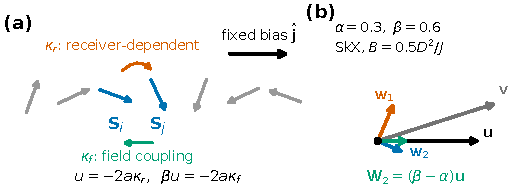
\includegraphics[width=\columnwidth]{fig1_concept.pdf}
\caption{\label{fig:concept}A current is a fixed nonreciprocal bond bias, and in the co-moving frame it enters only through two vectors of opposite time-reversal parity. (a) On a bond $i\to j$ the adiabatic term is a receiver-dependent coupling $\kappa_r$ and the $\beta$ term a field coupling $\kappa_f$ [Eq.~(\ref{eq:dictionary})]. (b) Slot vectors of the driven skyrmion lattice ($B=0.5D^2/J$, $\alpha=0.3$, $\beta=0.6$) from the exact Thiele projection: $\wone$ (T-odd) and $\wtwo$ (T-even) are perpendicular, and the Landau--Lifshitz drive $\Wtwo=(\beta-\alpha)\vu$ points along $\vu$ whatever the Hall angle of $\vv$.}
\end{figure}

%======================================================================
\section{Selection rules from the residual group}
\label{sec:groups}

The residual group of a driven pattern consists of the unitary elements $g$ with $R_g\wone=\wone$, $R_g\wtwo=\wtwo$ and the antiunitary elements $gT$ with $-R_g\wone=\wone$, $R_g\wtwo=\wtwo$. First-order response tensors must be covariant under it. Table~\ref{tab:groups} lists the magnetic point group, which decides the first-order modes, and the magnetic space group of a minimal commensurate realization, identified numerically by decorating every site with markers of $\wone$ and $\wtwo$ and analysing the result with spglib~\cite{spglib} (even period; orthorhombic host for one-dimensional patterns, hexagonal host for skyrmion lattices).

\begin{table*}[t]
\caption{\label{tab:groups}Residual magnetic groups of driven chiral patterns and the first-order modes they allow. BNS numbers refer to the minimal commensurate realization.}
\begin{ruledtabular}
\begin{tabular}{lllll}
Pattern & Bias & Residual point group & Residual space group (BNS) & First-order mode\\
\hline
N\'eel cycloid & none & $mm21'$ & $P_ama2$ (28.92) & --\\
& $\vu\parallel\mathbf q$ & $m'm2'$ & $Pm'a2'$ (28.89) & $M\parallel\hat z\times\vu$\\
& $\vu\perp\mathbf q$ & $mm'2'$ & $Pm'm2'$ (25.59) & none\footnotemark[1]\\
Bloch helix & none & $2221'$ & $P_c222_1$ (17.12) & --\\
& $\vu\parallel\mathbf q$ & $2'2'2$ & $P2'2'2_1$ (17.9) & $M\parallel\vu$\\
& $\vu\perp\mathbf q$ & $2'22'$ & $P2'2'2$ (16.3) & none\footnotemark[1]\\
N\'eel SkX & none & $6m'm'$ & $P6m'm'$ (183.189) & --\\
& $\wone\perp$ mirror & $m'$ & $Cm'$ (8.34) & $\mathbf d\perp\wone$\\
& generic & 1 & $P1$ & $\mathbf d\perp\wone$\footnotemark[2]\\
Bloch SkX & none & $62'2'$ & $P62'2'$ (177.153) & --\\
& $\wtwo\parallel 2'$ axis & $2'$ & $C2'$ (5.15) & $\mathbf d\perp\wone$\\
\end{tabular}
\end{ruledtabular}
\footnotetext[1]{$(\wone\cdot\nabla)\vm\equiv0$, so the unbiased pattern remains an exact solution.}
\footnotetext[2]{Fixed by linear response of the unbiased group.}
\end{table*}

\textit{Nonsymmorphic protection.} The elements that forbid an out-of-plane cone $M_z$ of a N\'eel cycloid with $\vu\parallel\mathbf q$ are the glide $m_yt_{\lambda/2}$ and the screw $2'_zt_{\lambda/2}$. Both exist only because a single-harmonic pattern is invariant under a half-period translation combined with time reversal, $Tt_{\lambda/2}$; for an incommensurate pattern this is the internal translation $(1'|0,0,0,\tfrac12)$ of its magnetic superspace group, so the rule holds in general. For a pattern locked to the lattice with an odd period the half translation is lost, the group drops to $Pm'$ (6.20), and $M_z$ appears as a weak lock-in effect. Space-group numbers depend on the host lattice; the point group and the nonsymmorphic generators are the robust statement.

\textit{Cone response: a pattern-mediated Edelstein effect.} For a harmonic helix, $\partial_q\vm=q\,\hat e\times\vm$ generates rotations about the axis $\hat e$, and its conjugate is the uniform cone magnetization $M$ along $\hat e$. With the cone energy $e(M)=-\Delta(1-M^2)$ the stationary condition $s\ueff q=\partial e/\partial M$ gives, for exchange plus DMI ($q=D/J$, $2\Delta=Dq$),
\begin{equation}
M=\frac{s\,\ueff}{D}.
\label{eq:cone}
\end{equation}
The cone scales with $(\beta/\alpha-1)$ and with $1/D$, and does not depend on the exchange stiffness. It points along $\hat z\times\vu$ in a N\'eel medium and along $\vu$ in a Bloch medium, the symmetry of the electronic Edelstein effect, and reverses with the chirality [Fig.~\ref{fig:patterns}(a)]. Because exchange plus DMI factorizes the cone energy as $1-M^2$, the pitch does not change at this order.

\textit{Skyrmion lattice.} Linear response of $6m'm'$ allows a dipolar distortion $\mathbf d=a\,\hat z\times\wone+b\,\wtwo$; since $\wtwo\perp\wone$, $\mathbf d\perp\wone$. Ellipse axes are parallel or perpendicular to $\wone$ (a $45^\circ$ tilt would need $\mathrm{sym}(\wone\otimes\wtwo)$, which $m'$ forbids), and the lowest orientational torque is $|\wone|^6\sin6(\theta-\phi_w)$, so a uniform current alone does not rotate the lattice~\cite{Everschor2012}. Figure~\ref{fig:symmetry} checks the distortion rule on driven stationary states: after the uniform translation is removed, the distortion axis stays perpendicular to $\wone$ within $1.5^\circ$ for three values of $\alpha$ and three current directions, while its angle to $\vu$ follows the Hall rotation.

\begin{figure}[t]
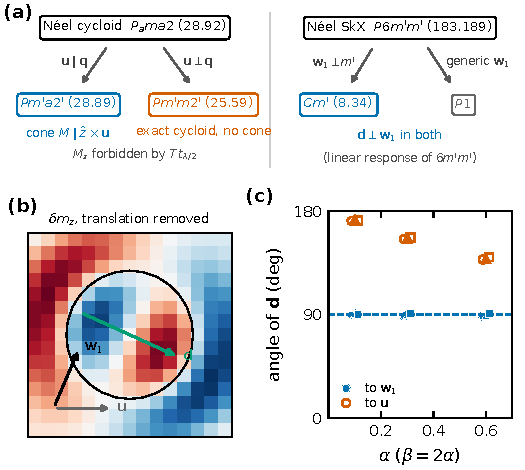
\includegraphics[width=\columnwidth]{fig2_symmetry.pdf}
\caption{\label{fig:symmetry}The residual magnetic group fixes the first-order response, and the vector that matters is $\wone$, not $\vu$. (a) Group--subgroup steps (BNS numbers). Cycloid: $\vu\parallel\mathbf q$ allows a uniform cone $M\parallel\hat z\times\vu$; $\vu\perp\mathbf q$ leaves the cycloid exact; $M_z$ is forbidden by $Tt_{\lambda/2}$. Skyrmion lattice: linear response of $6m'm'$ gives $\mathbf d\perp\wone$. (b) Change of $m_z$ of a driven N\'eel skyrmion ($\alpha=0.3$, $u=0.02$ along $x$) with the translation removed; contour $m_z=0$ of the static skyrmion; arrow the first moment $\mathbf d$ inside $r<5$. (c) Angle of $\mathbf d$ from $\wone$ (filled) and from $\vu$ (open) for $\alpha=0.1$, 0.3, 0.6 and current directions $0^\circ$, $30^\circ$, $90^\circ$.}
\end{figure}

%======================================================================
\section{Pattern Walker breakdown: unwinding versus the Landau criterion}
\label{sec:walker}

\textit{No precession.} The conjugate variable of a domain wall, its tilt angle, is periodic, so its restoring force is bounded and a strong enough drive makes the wall precess~\cite{SchryerWalker1974}. The conjugate variable of a pattern, the cone $M$, has a quadratic energy, so its restoring force grows without bound up to $|M|=1$ [Fig.~\ref{fig:walker}(a,b)]. The static branch therefore ends in one of two ways, whichever comes first: unwinding at $|M|=1$, $u_{\rm unw}=D/s$ for exchange plus DMI, or a Landau instability of the Goldstone mode,
\begin{equation}
\omega_0(k)<\lambda\,\ueff\,k .
\label{eq:landau}
\end{equation}

\textit{Origin of the criterion.} In the Landau--Lifshitz form a Bloch phonon $\Psi_k$ of the co-moving background has, to first order, the growth rate
\begin{equation}
\mathrm{Re}\,\lambda_k=-\alpha P_k\,\omega_k+\Wtwo\cdot\mathbf K^P_k ,
\label{eq:growth}
\end{equation}
where $P_k$ is the ellipticity of the mode and $\mathbf K^P_k$ its dissipative Doppler overlap, the shift of the damping rate per unit dissipative advection. The reactive slot $\mathbf W_1$ only shifts the real frequency at this order. Setting $\mathrm{Re}\,\lambda_k=0$ with $\Wtwo=(\beta-\alpha)\vu=\alpha\ueff\hat u$ gives Eq.~(\ref{eq:landau}) with
\begin{equation}
\lambda=\kP\equiv\frac{\hat u\cdot\mathbf K^P_k}{P_kk}
\label{eq:kP}
\end{equation}
(Appendix~\ref{app:identities}). The ellipticity cancels, so the criterion holds for overdamped modes too, and the Hall motion of the pattern does not enter because $\Wtwo\parallel\vu$. Damping enters only at order $\alpha^2$, through the deformation of the driven background and the mixing of the phonon with internal modes (Sec.~\ref{sec:tests}). $\omega_0$ is evaluated on the driven background.

\textit{Helix.} For exchange plus DMI with $\vu\parallel\mathbf q$ the compression phonon on the driven cone has the phase velocity $c=(D/s)\sqrt{1-M^2}$ and $\lambda=1$. With Eq.~(\ref{eq:cone}),
\begin{equation}
u_L=\frac{D}{\sqrt2\,s}<u_{\rm unw}=\frac{D}{s}:
\label{eq:uL}
\end{equation}
the helix always breaks by the Landau instability before it unwinds [Fig.~\ref{fig:walker}(c)]. With an easy-axis anisotropy $K$, writing $\Lambda=\sqrt{D^2+2AK}/s$ and $\kappa=D/\sqrt{D^2+2AK}$, one finds $u_L=\Lambda/\sqrt{1+\kappa^2}$ and $u_{\rm unw}=\Lambda/\kappa$, so $u_L<u_{\rm unw}$ for every $K$ [Fig.~\ref{fig:walker}(d)].

\textit{Dispersion order decides.} A linear Goldstone dispersion gives a finite threshold. A quadratic one, $\omega\simeq c_2k^2$, gives $\ueff^*=c_2k/\lambda\to0$, the reason why the Landau critical velocity of an ideal Bose gas vanishes~\cite{Landau1941}. This is the case for the gyrotropic magnetophonon of a skyrmion lattice~\cite{Petrova2011} and, in the continuum, for stripe bending. In a finite sample the threshold is set by the box, $\ueff^*\simeq2\pi c_2/(\lambda L)$, by a pinning gap of a sliding lattice, $\ueff^*=2\sqrt{\omega_{\rm pin}c_2}/\lambda$, or for stripes by the orientational stiffness of the host lattice. A statically pinned lattice depins first, 20--40 times below the sliding-lattice threshold (Appendix~\ref{app:pinning}).

\textit{Doppler efficiency.} If the phonon phase advances continuously through the texture (the affine limit), $\lambda=1$, and Eq.~(\ref{eq:landau}) reduces to the criterion of Okumura \textit{et al.} for skyrmion strings~\cite{Okumura2023}. If the phase advances in steps from skyrmion to skyrmion (the rigid-particle limit), $(\vu\cdot\nabla)$ does not act on it and $\lambda=0$: in a rigid Thiele model the current is a constant force that drops out of the phonon equation. Real patterns lie in between, and Sec.~\ref{sec:lambda} shows what sets $\lambda$.

\begin{figure}[t]
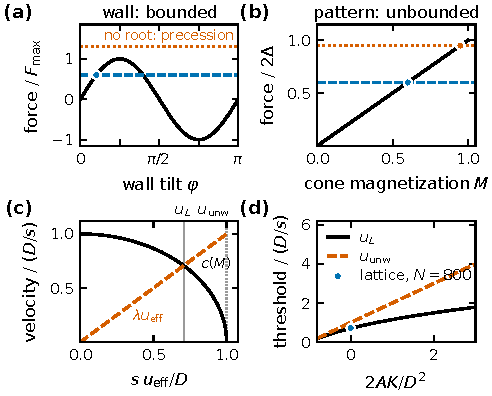
\includegraphics[width=\columnwidth]{fig3_walker.pdf}
\caption{\label{fig:walker}A pattern has no precessional Walker breakdown; its static branch ends in a Landau instability before it can unwind. (a) The tilt of a domain wall has a bounded restoring force; a drive above its maximum (dotted) has no static root. (b) The cone $M$ of a pattern has a linear restoring force up to $|M|=1$. (c) Helix: the compression velocity on the driven cone meets the Doppler line at $u_L=D/\sqrt2 s$, below $u_{\rm unw}=D/s$. (d) With easy-axis anisotropy $u_L<u_{\rm unw}$ for every $K$; point: exact Bloch threshold of an $N=800$ chain.}
\end{figure}

%======================================================================
\section{Tests: helix, skyrmion lattice, stripes}
\label{sec:tests}

All thresholds below are computed exactly from Bloch Jacobians of co-moving stationary states relaxed to a residual $\max|\dot\vm|<10^{-10}$ (one-dimensional patterns $<10^{-12}$; for skyrmion lattices the remaining residual of $\sim10^{-7}$ is a uniform translation from the frame velocity and changes growth rates by less than $10^{-7}$).

\textit{Helix.} The driven cone is exact on the lattice, $M=\ueff\sin\theta/[2(\sqrt{J^2+D^2}-J)]\to s\ueff/D$, with residual $10^{-15}$. For five pairs $(\alpha,\beta)$, including $\beta=0$ and $\beta<0$, the bare thresholds $u^*$ spread over a factor of two and both signs, while $\ueff^*$ agree to 0.1\% [Fig.~\ref{fig:helix}(a)]. Finite chains follow $\sqrt{(D^2+k_{\min}^2)/2}$, the Landau criterion at the smallest allowed wave number, and converge to $D/\sqrt2$ [Fig.~\ref{fig:helix}(b)].

\begin{figure}[t]
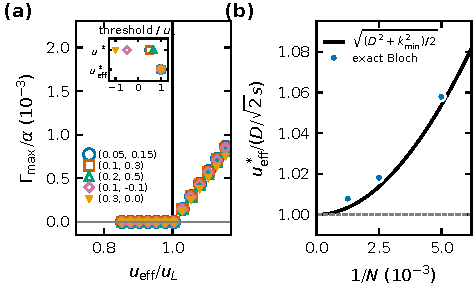
\includegraphics[width=\columnwidth]{fig4_helix.pdf}
\caption{\label{fig:helix}The driven helix breaks at $u_L=D/\sqrt2 s$ for every $(\alpha,\beta)$; $\beta$ enters only through $\ueff$. (a) Largest Bloch growth rate divided by $\alpha$ against $\ueff$ for five $(\alpha,\beta)$ ($N=200$; $u_L$ includes the finite-chain correction). Inset: the same thresholds in the bare current $u$ and in $\ueff$. (b) Exact thresholds of finite chains (points) against $\sqrt{(D^2+k_{\min}^2)/2}$ (line).}
\end{figure}

\textit{Skyrmion lattice.} We use a square lattice with $D=0.4$ and a $19\times33$ cell holding two skyrmions. At $B=0.5D^2/J$ the threshold is proportional to $k$, $\ueff^*=0.0101$, 0.0203, 0.0405, 0.081 at $k=0.0083$, 0.0165, 0.033, 0.066, and agrees with $c_2k/\kP$ to 0.4--0.9\% without fitting; the affine estimate $c_2k$ is off by a factor of two [Fig.~\ref{fig:skx}(a)]. Over four fields $\lambda$ falls from 0.77 to 0.11 and follows the dissipative overlap $\kP$, not the reactive overlap $\kt$ [Fig.~\ref{fig:skx}(b), Table~\ref{tab:lambda}]. The damping dependence is quadratic, $\Delta\lambda/\lambda=-c(\alpha^2-\alpha_0^2)$ with $c=-0.08$, 0.10, 0.33, 0.54 for $B=0.3$, 0.5, 0.7, 0.85 [Fig.~\ref{fig:skx}(c)], so for $\alpha\le0.1$ the threshold equals $c_2k/\kP$ within 0.6\%. The sign of $c$ follows $\kP-\kt$: the leading correction is a cross term $(w_{1x}/\ueff)(\kt-\kP)=O(\alpha^2)$ between damping and the Hall residual of the reactive slot, plus deformation of the driven background and mixing with internal modes of the same order (Appendix~\ref{app:identities}). At $\alpha=0.6$ the phonon is near critical damping ($\alpha P\approx1$), and we restrict quantitative statements to $\alpha\le0.3$.

\begin{table}[b]
\caption{\label{tab:lambda}Skyrmion lattice ($19\times33$, $k=0.0165$, $\beta=2\alpha$): phonon velocity $\omega/k$, overlaps, ellipticity and the Doppler efficiency $\lambda=\omega/(k\ueff^*)$ from exact thresholds.}
\begin{ruledtabular}
\begin{tabular}{ccccccc}
$B$ $(D^2/J)$ & $\omega/k$ & $\kP$ & $\kt$ & $P$ & $\lambda_{\alpha=0.05}$ & $\lambda_{\alpha=0.3}$\\
\hline
0.30 & 0.01195 & 0.773 & 0.862 & 1.95 & 0.774 & 0.779\\
0.50 & 0.01018 & 0.505 & 0.451 & 1.70 & 0.506 & 0.502\\
0.70 & 0.00588 & 0.226 & 0.142 & 1.58 & 0.228 & 0.222\\
0.85 & 0.00315 & 0.107 & 0.047 & 1.55 & 0.109 & 0.104\\
\end{tabular}
\end{ruledtabular}
\end{table}

\begin{figure}[t]
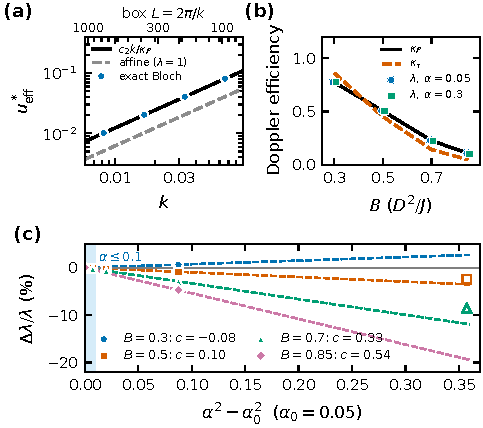
\includegraphics[width=\columnwidth]{fig5_skx.pdf}
\caption{\label{fig:skx}The skyrmion-lattice threshold is $\ueff^*=c_2k/\lambda$ with $\lambda=\kP$; damping enters only at order $\alpha^2$. (a) Exact Bloch thresholds ($B=0.5D^2/J$, $\alpha=0.3$, $\beta=0.6$) against $c_2k/\kP$ (line) and the affine estimate (dashed); top axis the box length $L=2\pi/k$. (b) $\lambda$ from exact thresholds at $\alpha=0.05$ and 0.3 against $\kP$ (solid) and $\kt$ (dashed). (c) $\Delta\lambda/\lambda$ against $\alpha^2-\alpha_0^2$, fitted for $\alpha\le0.3$ (filled); open symbols $\alpha=0.6$; shaded $\alpha\le0.1$.}
\end{figure}

\textit{Real-time breakdown.} The Bloch analysis predicts the dynamics directly. In a $76\times66$ box (16 skyrmions) at $\ueff=0.15$, 1.5 times the threshold of the $k_1=2\pi/76$ mode, the satellite $|m_z(k_1)|$ grows from noise at exactly the Bloch rate of that mode, $\Gamma=7.26\times10^{-4}$, without any fitted slope, while at $\ueff=0.05$ the noise decays [Fig.~\ref{fig:breakdown}(a,b)]. The growing mode is a box-length wave of skyrmion displacements along the current; once it saturates the lattice disorders without losing skyrmions. In a $76\times33$ box, lab-frame, Bloch and overlap thresholds agree within 4\% (0.0995, 0.1016, 0.1031), while the affine estimate (0.049) is off by a factor of two and the rigid-particle picture predicts no instability at all.

\begin{figure}[t]
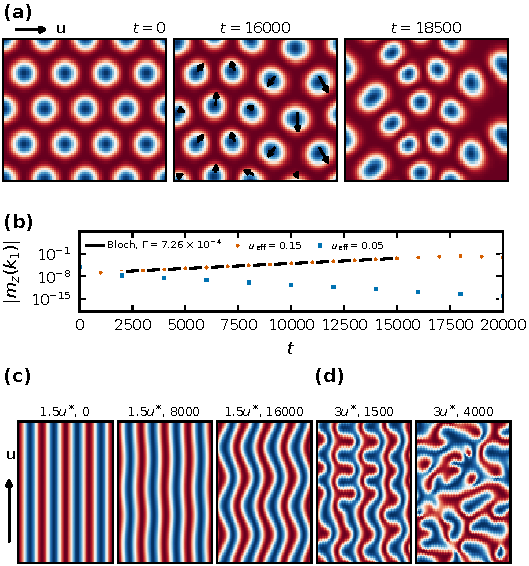
\includegraphics[width=\columnwidth]{figP2_breakdown.pdf}
\caption{\label{fig:breakdown}Above the Doppler threshold the Goldstone mode grows at the Bloch rate and then reorganizes the pattern. (a) Skyrmion lattice at $\ueff=0.15$ (1.5 times threshold; $76\times66$, co-moving frame); arrows at $t=16000$: skyrmion displacements since $t=0$ ($\times4$). (b) $|m_z(k_1)|$ against time (points) and the Bloch growth rate of the same mode (line, no fit); below threshold ($\ueff=0.05$) the noise decays. (c) Stripes ($P=30$) driven along themselves at $1.5u^*$: the longest bending wave grows and saturates into a zigzag. (d) At $3u^*$: shorter waves, dislocations and a labyrinth. The late stages are treated in Ref.~\cite{B2}.}
\end{figure}

\textit{Stripes.} On the square lattice a stripe with $\mathbf q\parallel\hat x$ is an orientational saddle, so we use the stable diagonal orientation with periods $P=30$, 60, 120. The bending branch (wave vector along the stripes) has no gap,
\begin{equation}
\omega^2=c_0^2(1-\eta M^2)k^2+c_b^2k^4 ,
\label{eq:stripe}
\end{equation}
where $c_0=0.0635$, 0.0165, 0.0048 for $P=30$, 60, 120 vanishes as $D^{1.9}$: the linear term is a lattice-anisotropy effect, and in the continuum stripes have a quadratic Goldstone mode like the skyrmion lattice; $c_b\to0.52$. A current component along $\mathbf q$ builds the cone $M=s\ueff\cos\varphi/D$ ($\varphi$ is the angle between $\vu$ and $\mathbf q$) and only scales the bending velocity. Measured mode by mode, the ratio $\omega(k;M)/\omega(k;0)$ is the same for every $k$ in the long-wave range and gives $\eta=1.40$ for both $P=30$ and 60 [Fig.~\ref{fig:stripes}(a)]. The $k$ independence is what the conjugacy of the stripe phase and the cone requires (Appendix~\ref{app:stripe}); the value of $\eta$, larger than the exchange value 1, reflects the anisotropic origin of $c_0$. With the Doppler projection $\ueff\sin\varphi$ on the stripe direction and $\lambda=1$, the Landau criterion at $k\to0$ gives
\begin{equation}
\ueff^*=\frac{c_0}{\sqrt{\sin^2\varphi+\eta(c_0/D)^2\cos^2\varphi}},
\label{eq:stripe_threshold}
\end{equation}
which reproduces the exact thresholds at $\varphi=90^\circ$, $60^\circ$, $30^\circ$ [Fig.~\ref{fig:stripes}(b)] and tends to the unwinding point $D$ as $\varphi\to0$. In a box of length $L$ along the stripes the longest bending mode sets $\ueff^*\sin\varphi=\sqrt{c_M^2+(2\pi c_b/L)^2}$ with $c_M=c_0\sqrt{1-\eta M^2}$; dynamical thresholds in sheared boxes of $L=64$--512 collapse onto this form for both periods and all three angles [Fig.~\ref{fig:stripes}(c)], except where the box wave number approaches the stripe wave number ($P=60$, $L=64$). Above threshold the longest bending wave grows first, its wave number rising as $\sqrt{u/u^*-1}$ near threshold and $\propto u$ far above, as reported for helices~\cite{Masell2020}, and saturates into a zigzag at $1.5u^*$ [Fig.~\ref{fig:breakdown}(c,d)].

\begin{figure}[t]
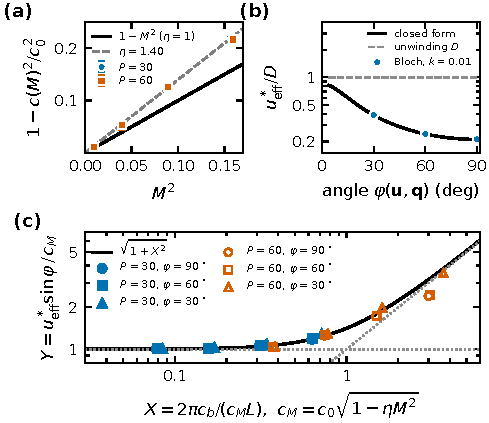
\includegraphics[width=\columnwidth]{fig6_stripes.pdf}
\caption{\label{fig:stripes}Stripes have a quadratic Goldstone mode; a current along $\mathbf q$ only scales the bending velocity, and finite-box thresholds collapse. (a) $1-c(M)^2/c_0^2$ against $M^2$ from the $k$-resolved ratio $\omega(k;M)/\omega(k;0)$ (error bars: spread over $k$); $\eta=1.40$ for $P=30$ and 60. (b) Threshold against the current angle ($P=30$): exact Bloch thresholds at $k=0.01$ and Eq.~(\ref{eq:stripe_threshold}). (c) Dynamical thresholds in boxes of length $L$, $P=30$ (filled) and 60 (open), collapse onto $Y=\sqrt{1+X^2}$.}
\end{figure}

%======================================================================
\section{What sets the Doppler efficiency}
\label{sec:lambda}

\textit{Two metrics, one mode.} Two exact identities of the linearized Gilbert operator $J$ at $\alpha=0$,
\begin{equation}
\frac{\partial J}{\partial\wtwo}=-\Omega\,\frac{\partial J}{\partial\wone},\qquad \frac{\partial J}{\partial\alpha}=-\Omega J,
\label{eq:identities}
\end{equation}
with $\Omega$ the symplectic form of the tangent plane (Appendix~\ref{app:identities}), turn both Doppler overlaps into momenta of the same Bloch mode $\psi$, measured in two metrics:
\begin{gather}
\kt=\frac{\langle\psi|\Omega\Pg|\psi\rangle}{k\langle\psi|\Omega|\psi\rangle},\qquad
\kP=\frac{\langle\psi|\Pg|\psi\rangle}{k\langle\psi|\psi\rangle},\nonumber\\
P=\frac{\langle\psi|\psi\rangle}{|\langle\psi|\Omega|\psi\rangle|},
\label{eq:overlaps}
\end{gather}
where $\Pg$ is the advection (momentum) generator. $\kt$ is the momentum in the symplectic (Berry) metric and sets the reactive Doppler shift; $\kP$ is the momentum in the dissipative metric and sets the threshold.

\textit{Static theorem.} Write the Bloch mode as $\Psi_k=e^{ikx}(\phi_G+k\phi_1)$, with $\phi_G$ the Goldstone mode. $\lambda$ is fixed by the corrector $\phi_1$. The identity $[H_0,x]=-i\partial_kH_k$ makes $\phi_1=-ix\phi_G$ an exact solution except at cell boundaries, so $\lambda=0$ when $\phi_G$ vanishes between pattern units (the rigid limit) and $\lambda=1$ when the texture is uniform. For a type-B Goldstone mode ($\omega\propto k^2$) the dynamical term is $O(k^2)$, so the $O(k)$ corrector solves a static problem: both overlaps equal those of the statically relaxed strain mode and are independent of the dynamics and of $\alpha$. Table~\ref{tab:static} confirms this for seven lattices.

\textit{One-dimensional theorem.} If the conjugate field of the in-plane angle $\theta$ is slaved locally by a strong easy-plane anisotropy, a ground-state transformation maps the problem onto homogenization with conductivity $\sigma=\psi_0^2$, $\psi_0=\theta_0'$, and
\begin{equation}
\lambda=\frac{1}{\langle\psi_0^2\rangle\langle\psi_0^{-2}\rangle}
\label{eq:homog}
\end{equation}
(with a nonuniform conjugate stiffness $M(x)$, $\langle M^{-1}\rangle/[\langle\psi_0^{-2}\rangle\langle\psi_0^2/M\rangle]$). A uniform helix gives $\lambda=1$; a dilute soliton lattice gives $\lambda\propto e^{-L/w}$ with $w=\sqrt{J/B}$. For a chiral soliton lattice~\cite{Kishine2015} Eq.~(\ref{eq:homog}) agrees with the exact overlap within 2\% at nine fields, and fails as it should when the conjugate field is not slaved [Fig.~\ref{fig:lambda}(a)].

\begin{table}[t]
\caption{\label{tab:static}Static theorem and two-field theory: dynamic, static and two-field values of both overlaps for seven skyrmion lattices (cell width $a$, field $B$ in $D^2/J$).}
\begin{ruledtabular}
\begin{tabular}{ccccccc}
 & \multicolumn{3}{c}{$\kP$} & \multicolumn{3}{c}{$\kt$}\\
$a$, $B$ & dyn. & static & two-field & dyn. & static & two-field\\
\hline
19, 0.3 & 0.773 & 0.775 & 0.779 & 0.862 & 0.862 & 0.863\\
19, 0.5 & 0.505 & 0.506 & 0.507 & 0.451 & 0.453 & 0.453\\
19, 0.7 & 0.226 & 0.227 & 0.225 & 0.142 & 0.143 & 0.145\\
19, 0.85 & 0.107 & 0.107 & 0.111 & 0.047 & 0.047 & 0.050\\
13, 0.5 & 0.228 & 0.229 & 0.234 & 0.104 & 0.105 & 0.104\\
15, 0.5 & 0.327 & 0.327 & 0.332 & 0.217 & 0.219 & 0.218\\
23, 0.6 & 0.339 & 0.340 & 0.337 & 0.282 & 0.284 & 0.287\\
\end{tabular}
\end{ruledtabular}
\end{table}

\textit{Counterflow.} Figure~\ref{fig:counterflow} shows what the static corrector does. Under a long-wave strain the affine mode squeezes and stretches the skyrmions with the lattice; the relaxed mode with the same skyrmion displacements keeps them round, and the difference between the two is a pattern of spin canting at the skyrmion cores. This canting carries a Berry-phase momentum that cancels part of the Doppler momentum of the affine mode: at a wavelength of two cells the momentum per $k$ drops from 0.95 to 0.72 at $B=0.3$ and from 0.93 to 0.07 at $B=0.85$. Hence, with $\Pi_{\rm cf}$ the counterflow momentum (per unit affine momentum) carried by the internal relaxation,
\begin{equation}
\lambda=1-\Pi_{\rm cf},
\label{eq:counterflow}
\end{equation}
the analogue of Feynman backflow or of a $k\cdot p$ effective mass. A two-field Ritz theory with the displacement envelope and its spin-conjugate canting envelope, without fitted parameters, reproduces both overlaps of all seven lattices to $\pm0.01$, while displacement-only theories and the affine mode do not [Table~\ref{tab:static}, Fig.~\ref{fig:lambda}(b)]. The canting is only 4--16\% of the corrector norm but carries a large momentum, because $\lambda$ is a cross term between displacement and canting; the counterflow is a magnetic, not an elastic, effect. Projecting the corrector on local channels shows that the helicity twist is always rigid, because DMI locks the helicity, and that $\lambda$ follows the affinity of the elliptic (shear) channel. Soft ellipse modes reverse the counterflow and give $\lambda>1$ (1.69 at $a=23$, $B=0.4$).

\textit{Why $\kP>\kt$ in dilute lattices.} Split $\psi$ into its co-rotating and counter-rotating tangent-plane components (eigenvectors of $\Omega$) with momenta per norm $\pi_\pm$. The dissipative metric adds the two components and the symplectic metric subtracts them (Appendix~\ref{app:circular}). The counterflow cancels mainly the co-rotating, gyrotropic momentum, $\pi_+=0.80\to0.08$ for $B=0.3\to0.85$, while the counter-rotating admixture keeps more, $\pi_-=0.68\to0.22$ [Fig.~\ref{fig:lambda}(c)], so $\kP>\kt$ exactly when $\pi_->\pi_+$.

\begin{figure}[t]
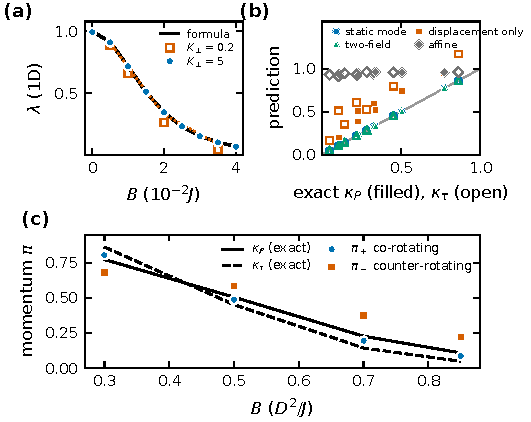
\includegraphics[width=\columnwidth]{fig7_lambda.pdf}
\caption{\label{fig:lambda}$\lambda$ is a static property: one minus the counterflow momentum of the internal relaxation. (a) Chiral soliton lattice: exact overlap against Eq.~(\ref{eq:homog}) with a slaved conjugate field ($K_\perp=5$); with $K_\perp=0.2$ the formula (dotted) overestimates $\lambda$. (b) Seven skyrmion lattices: predictions against exact $\kP$ (filled) and $\kt$ (open). (c) Momenta of the co-rotating ($\pi_+$) and counter-rotating ($\pi_-$) components with the exact overlaps.}
\end{figure}

\begin{figure}[t]
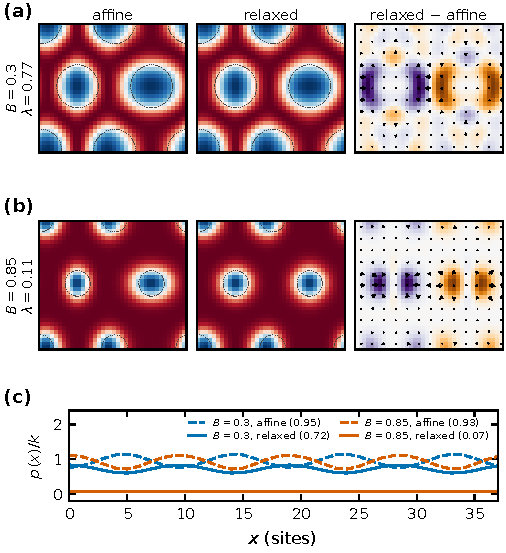
\includegraphics[width=\columnwidth]{figP3_counterflow.pdf}
\caption{\label{fig:counterflow}$\lambda$ in real space. (a, b) A longitudinal strain wave (wavelength two cells, displacement amplitude 2 sites, exaggerated) at $B=0.3D^2/J$ ($\lambda=0.77$) and $0.85D^2/J$ ($\lambda=0.11$). Left: affine mode; middle: statically relaxed mode with the same displacement; right: their difference, the internal canting (colour $\delta m_z$, arrows in-plane). Dotted: $m_z=0$ of the undeformed lattice. (c) Doppler-momentum density of the phonon averaged across the strip, divided by $k$; averages in brackets.}
\end{figure}

%======================================================================
\section{Below threshold: a moving Gibbs ensemble}
\label{sec:gibbs}

Inserting the Doppler term into the dynamics of the gyrotropic displacement field gives an effective energy $E-\vv\cdot\Pg$ with $\vv=\lambda\ueff\hat u$. Its pseudo-momentum term is a Lifshitz invariant of the displacement field with coefficient $(G/2)\lambda(\beta-\alpha)u/\alpha$ (Appendix~\ref{app:gibbs}), a ``DMI of the lattice displacement''. A phonon carries pseudo-momentum $\pm k$, so the two branches at the same $k$ carry effective temperatures
\begin{equation}
T_{\rm eff}=\frac{T}{1\mp x},\qquad x=\frac{\lambda\ueff k}{\omega_k},
\label{eq:Teff}
\end{equation}
and the Landau threshold $x=1$ is where this ensemble stops being normalizable. Because the displacement field is real, the branches $(k,\omega)$ and $(-k,\omega)$ are conjugate and the damping rates obey the sum rule $\Gamma_++\Gamma_-=2\Gamma_0$ to first order; numerically $\Gamma_++\Gamma_-=0.834+2.551=3.385$ against $2\Gamma_0=3.388$ (same units) at $k_1$ and $\ueff=0.05$, and the deviations grow as $u^2$.

Stochastic LLG simulations at $k_BT=0.01$ test Eq.~(\ref{eq:Teff}). At $k_1=2\pi/76$ the two branches follow $1/(1\mp x)$ up to $x=0.7$ [Fig.~\ref{fig:gibbs}(a)]. In a $152\times66$ box at $\ueff=0.03$, modes along the current heat as $1/(1-x^2)$ while transverse and oblique modes stay at the bath temperature [Fig.~\ref{fig:gibbs}(b)]; since $x\propto k_\parallel/k^2$, heating concentrates in the longest wavelengths along the current.

\textit{Melting.} Heating ladders of 256--264 skyrmions give $T_m(0)=0.201\pm0.002$, close to the KTHNY estimate from the elastic constants~\cite{HalperinNelson1978,Young1979}. A current below threshold barely moves it, $T_m(u)/T_m(0)=0.97$--1.00 within errors of 0.01--0.05, although the longest mode of the larger box is already at $x=0.89$ [Fig.~\ref{fig:gibbs}(c)]. Melting is controlled by bond-scale strain fluctuations, to which every mode contributes equally by equipartition, so the relevant measure is the Brillouin-zone average
\begin{equation}
\frac{\Delta\langle\varepsilon^2\rangle}{\langle\varepsilon^2\rangle}=\Big\langle\frac{1}{1-x_k^2}\Big\rangle_{\rm BZ}-1\approx\Big(\frac{\lambda\ueff}{c_2}\Big)^2\frac{\pi\ln(k_{\max}/k_{\min})}{A_{\rm BZ}} ,
\label{eq:zone}
\end{equation}
which is 3.5\% and 6.6\% for the two boxes at $\ueff=0.03$ and agrees with the measured shifts; a criterion based on the longest modes predicts 24--40\% and is ruled out. Because a lattice below threshold has $\ueff\le c_2k_{\min}/\lambda$, Eq.~(\ref{eq:zone}) is bounded by $\pi A_{\rm cell}\ln(Lk_{\max}/2\pi)/L^2$, which vanishes for large $L$: below the Doppler threshold a current cannot lower the melting temperature of a large sample appreciably. Far above threshold the current melts the lattice into a flowing skyrmion liquid~\cite{B2}.

\begin{figure}[t]
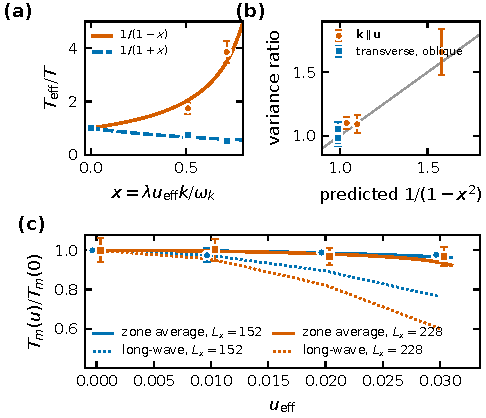
\includegraphics[width=\columnwidth]{fig8_gibbs.pdf}
\caption{\label{fig:gibbs}Below threshold the current puts the lattice phonons in a Gibbs ensemble moving at $\lambda\ueff$, and the melting point moves only by the zone average of that heating. (a) Effective temperatures of the two branches at $k_1=2\pi/76$ ($76\times33$, $k_BT=0.01$) against $1/(1\mp x)$. (b) Variance ratio of displacement modes ($152\times66$, $\ueff=0.03$) against $1/(1-x^2)$. (c) Melting temperature against $1/\langle(1-x^2)^{-1}\rangle_{\rm BZ}$ (solid) and the long-wave criterion (dotted) for two box shapes.}
\end{figure}

%======================================================================
\section{Beyond current: nonreciprocal DMI and damping-like spin--orbit torque}
\label{sec:sot}

\textit{Exchange-parity rule.} A first-order nonreciprocal DMI has $\mathbf n_{ji}=\mathbf n_{ij}$, so it is even in the bond direction. The neighbour sum $\sum_{\hat e}\mathbf n\times(\mathbf S_{i+\hat e}+\mathbf S_{i-\hat e})\approx\sum_{\hat e}\mathbf n\times(2\mathbf S_i+\partial_{\hat e}^2\mathbf S)$ then has no first-gradient term: an exchange-odd coupling ($\delta J$) advects, which is the Zhang--Li case, while an exchange-even one ($\delta D$) acts locally plus through a second-order nonreciprocal stiffness. Its time-reversal-even channel is a damping-like torque $-\mathbf S\times(\mathbf S\times\mathbf n)$, i.e., damping-like spin--orbit torque (SOT)~\cite{Manchon2019}; its odd channel is a field-like torque. In a N\'eel medium the map $\mathbf n\leftrightarrow\hat z\times\mathbf p$ gives a field-like $\mathbf n$ the residual group of $\wone$ and a damping-like $\mathbf n$ that of $\wtwo$.

\textit{Damping-like SOT pumps with zero threshold.} The field-like torque neither moves the lattice nor pumps (damping rates change by less than 0.05\%). The damping-like torque ($c=0.004$, $\mathbf n=\hat y$) makes the lattice flow and pumps modes with $\mathbf k$ close to $\hat z\times\mathbf n$, with $x\cdot k$ nearly constant, so $x\propto1/k$ and the threshold vanishes in an infinite system [Fig.~\ref{fig:sot}(a)]. The mechanism is not advection: pure drift cancels the Doppler term because its dissipative slot vanishes. An exact first-order decomposition shows that the pumping is a strain-dependent force; applied to the static relaxed mode the SOT generator reproduces the exact pumping coefficient at every $k$, and applied to the affine mode it gives exactly zero [Fig.~\ref{fig:sot}(b)].

\textit{Duality.} Zhang--Li acts fully on the affine part, and the internal relaxation reduces it ($\lambda<1$). Damping-like SOT gives zero on the affine part, and the internal relaxation alone produces the pumping. Both are overlaps of a nonreciprocal generator on the same static relaxed mode, so $\lambda$ and the SOT pumping coefficient are static material quantities of the same kind. At equal lattice velocity SOT pumps about 1.7 times more strongly than the current.

\textit{Second-order nonreciprocal stiffness.} The full exchange-even coupling contains, beyond its local Zeeman-like part, the stiffness $T_2=\delta D\,P_\perp(\mathbf n\times\nabla^2\mathbf S)$. It is odd in $\mathbf S$, hence reactive, and non-variational, so unlike a translation-invariant energy it exerts a net force on a pattern, $\mathbf F\parallel\mathbf n$ for a N\'eel lattice (Appendix~\ref{app:force}); the Thiele response $(G-\alpha\Dm)\vv=\mathbf F$ reproduces the measured drift to three digits. On a modulated background $\nabla^2$ acts on a phonon envelope as $2i\mathbf k\cdot\nabla$, so $T_2$ contains a $k$-linear Doppler term although the coupling is even in the bond direction: for $\mathbf k\perp\mathbf n$ a frequency shift that damping converts into a splitting, for $\mathbf k\parallel\mathbf n$ an intrinsic splitting carried by the static relaxed mode. Both splittings are $\propto k$ while the bare damping is $\propto k^2$, so the threshold $\delta D^*\propto k$ vanishes [Fig.~\ref{fig:sot}(c)]: a second route to zero-threshold pumping that needs no current.

\begin{figure}[t]
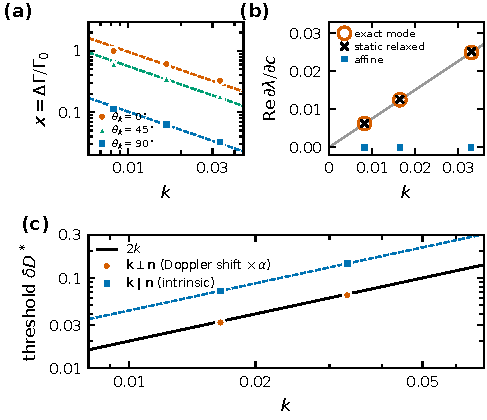
\includegraphics[width=\columnwidth]{fig9_sot.pdf}
\caption{\label{fig:sot}Exchange-even couplings pump with zero threshold through the static relaxed mode, dual to the Zhang--Li Doppler term. (a) Damping-like SOT ($c=0.004$, $\mathbf n=\hat y$, $\alpha=0.3$): pumping ratio $x=\Delta\Gamma/\Gamma_0$ for three directions of $\mathbf k$; dashed $1/k$. (b) First-order SOT generator on the exact, static relaxed and affine modes ($\alpha=0$). (c) Nonreciprocal DMI stiffness: threshold $\delta D^*$ for $\mathbf k\perp\mathbf n$ and $\mathbf k\parallel\mathbf n$; both $\propto k$.}
\end{figure}

%======================================================================
\section{Where the model meets real samples}
\label{sec:real}

The Landau criterion~(\ref{eq:landau}) rests on two assumptions: the adiabatic torque has the structure of advection, and damping acts as friction against the lattice. Both follow from the form of the Zhang--Li torque and of Gilbert damping, not from microscopic details, so the threshold is set by the ratio of $\ueff$ to the DMI velocity $D/s$ and by two properties of the pattern, the order of its Goldstone dispersion and $\lambda$. Real magnets have $\alpha\lesssim0.1$, where $\lambda=\kP$ within 0.6\%, so $\lambda$ can be computed from the static pattern alone. The velocity scale is $D/s=\gamma D/M_s$; with $\ueff=(\beta/\alpha-1)u$ and $u=g\mu_BPj/(2eM_s)$, the helix threshold $u_L=D/\sqrt2s$ corresponds to
\begin{equation}
j_L=\frac{\sqrt2\,e\gamma D}{g\mu_BP}\,\frac{\alpha}{\beta-\alpha},
\label{eq:jL}
\end{equation}
independent of $M_s$ and of the exchange stiffness. The predictions, written as dependencies, are:
\begin{itemize}
\item The cone magnetization $M/M_s=s\ueff/D$ grows with $\beta/\alpha-1$ and $1/D$, along $\hat z\times\mathbf j$ in N\'eel and along $\mathbf j$ in Bloch media, and reverses with the chirality, consistent with the sign rule observed in MnP~\cite{Jiang2020}.
\item The helix breaks at $j_L\propto D\alpha/(\beta-\alpha)$, Eq.~(\ref{eq:jL}), a factor $1/\sqrt2$ below the point where the cone would close~\cite{Masell2020}.
\item Skyrmion lattices flow stably in small samples because their threshold rises as $1/L$; in weakly pinned sliding lattices it is $2\sqrt{\omega_{\rm pin}c_2}/\lambda$.
\item The skyrmion-lattice threshold rises with field as $c_2/\lambda$, because skyrmions become particle-like and $\lambda$ falls.
\item The threshold is insensitive to damping and to the skyrmion Hall angle at fixed $\ueff$; changes are of order $\alpha^2$.
\item Stripes are destabilized by any current component along them, with a threshold that vanishes as $1/L$, the longest bending wave going first; a component along $\mathbf q$ only softens the bending velocity by $\sqrt{1-\eta M^2}$.
\item Distortions and ellipse axes of a driven skyrmion lattice lock to the Hall-rotated $\wone$, not to $\mathbf j$.
\item Below threshold the longest phonons along the current are hot, $T_{\rm eff}=T/(1-x)$, visible in their spectra, while the melting temperature moves only by the zone average, a few percent.
\end{itemize}

%======================================================================
\section{Conclusion}
\label{sec:conclusion}

A nonreciprocal spin coupling with a fixed direction, whether produced by a current or designed, acts on a chiral pattern through one structure: two vectors of opposite time-reversal parity in the co-moving stationary equation, whose dissipative combination is exactly $(\beta-\alpha)\vu$. This structure fixes which distortions a driven pattern may develop, rules out a precessional Walker breakdown and replaces it with a Doppler instability of the pattern's own Goldstone mode. Whether a pattern survives a finite current is decided by the order of its Goldstone dispersion; how strongly the current couples to that mode is decided by a static property, the Doppler efficiency $\lambda$, which measures how continuously the pattern phase advances and is set by the counterflow of strain-induced spin canting. Exchange-even couplings reach the same modes through the dual route. What a pattern does beyond its threshold is the subject of Ref.~\cite{B2}.

\begin{acknowledgments}
This research was supported by the National Research Foundation (NRF) of Korea funded by the Korean Government (NRF-2023R1A2C1006050).
\end{acknowledgments}

\section*{Data availability}
The code and data that reproduce every figure are available at \url{https://github.com/cywon-commits/NonReciprocalInteraction_SelfOrganizedPattern} (branch \texttt{b1/request6}, folders \texttt{figs\_b1} and \texttt{results/b1\_figs}).

%======================================================================
\appendix

\section{Operator identities and the Landau criterion}
\label{app:identities}

Linearize the Gilbert equation about a co-moving stationary state in the local tangent frame with symplectic form $\Omega$ ($\Omega^2=-1$), and write $J(\wone,\wtwo,\alpha)$ for the Bloch Jacobian at wave vector $k$. Because $\vm\times$ acts on the tangent plane as $-\Omega$ and the Gilbert form gives $\partial_t\vm=(\mathbf T+\alpha\vm\times\mathbf T)/(1+\alpha^2)$, the identities~(\ref{eq:identities}) hold exactly at $\alpha=0$; we verified them numerically to $10^{-10}$. For a Hamiltonian Bloch mode $J\psi=i\omega\psi$, first-order perturbation theory with left vector $\Omega^T\psi$ gives
\begin{equation}
\delta\lambda=-i\,w_{1x}k\kt+w_{2x}Pk\kP-\alpha P\omega .
\end{equation}
The reactive slot shifts only the frequency, and damping then acts on the shifted frequency. Writing $\wtwo=\Wtwo-\alpha\wone$ with $\Wtwo=\alpha\ueff\hat x$ gives
\begin{gather}
\mathrm{Re}\,\lambda=\alpha P\big[\lambda\ueff k-\omega\big],\nonumber\\
\lambda=\kP+\frac{w_{1x}}{\ueff}(\kt-\kP)+O(\alpha^2)_{\rm bg}.
\end{gather}
The exact Thiele solution gives $w_{1x}=\alpha\Dm^2(\beta-\alpha)u/(G^2+\alpha^2\Dm^2)$, so the cross term is of order $\alpha^2$; ``bg'' marks terms of the same order from the deformation of the driven background and from second-order mixing with internal modes. The leading term $\lambda=\kP$ is independent of $\alpha$, of $\beta$ beyond $\ueff$, and of the Hall angle.

\section{Moving Gibbs ensemble}
\label{app:gibbs}

Project the stochastic LLG on the pumped mode $a_k$. With the growth rate of Appendix~\ref{app:identities} and a bath noise fixed by Gilbert damping (fluctuation--dissipation at temperature $T$ for the undriven rate $\Gamma_0=\alpha P\omega$),
\begin{equation}
\dot a_k=\big[i\omega_k-\Gamma_0(1-x)\big]a_k+\xi_k,\qquad \langle\xi_k\xi_k^*\rangle=2\Gamma_0\frac{T}{\varepsilon_k},
\end{equation}
so $T_{\rm eff}=T/(1-x)$, and the conjugate branch has $1+x$. The stationary distribution is $\exp[-(E-\vv\cdot\Pg)/T]$ with $\vv=\lambda\ueff\hat x$ and $\Pg$ the pseudo-momentum of the gyrotropic displacement field $\mathbf u(\mathbf r)$. For a type-B mode $\varepsilon_k/\omega_k=G|u_k|^2$, so
\begin{equation}
E-\vv\cdot\Pg=E-\frac{G}{2}\lambda\frac{\beta-\alpha}{\alpha}u\int d^2r\,(u_x\partial_xu_y-u_y\partial_xu_x),
\end{equation}
a Lifshitz invariant of the displacement field. The derivation needs the noise projection to be unchanged at $O(u)$, which holds for $\alpha\le0.3$.

\section{Stripe bending threshold}
\label{app:stripe}

With Eq.~(\ref{eq:stripe}) and the Doppler projection $\ueff\sin\varphi$, $\min_k\omega/k$ is reached at $k\to0$, at $c_0\sqrt{1-\eta M^2}$ with $M=s\ueff\cos\varphi/D$; solving gives Eq.~(\ref{eq:stripe_threshold}). The stripe phase $\theta$ and the cone $M$ are conjugate, and for exchange plus DMI the cone energy $-\Delta(1-M^2)$ has the $M$-independent curvature $2\Delta$. A phase stiffness that is quadratic in the rotating amplitude $r=\sqrt{1-M^2}$ then gives $\omega^2=(r^2K_\theta k^2)(2\Delta)/s^2$: every such phase velocity scales by the same factor, independent of $k$, as the helix compression velocity $(D/s)\sqrt{1-M^2}$ does. The lattice bending stiffness $c_0^2$ comes from the orientational anisotropy of the host lattice, whose dependence on $r$ need not be quadratic; the measured factor is $k$-independent, as the conjugacy requires, with $\eta=1.40$. In the continuum $c_0\to0$, and a box of length $L$ along the stripes gives $\ueff^*\sin\varphi=2\pi c_b/L$.

\section{Pinning}
\label{app:pinning}

A weak pinning potential adds $K_{\rm pin}$ to both elastic eigenvalues of the displacement field, so $\omega(k)\approx\omega_{\rm pin}+c_2k^2$ and the Landau minimum at $k^*=\sqrt{\omega_{\rm pin}/c_2}$ gives $\ueff^*=2\sqrt{\omega_{\rm pin}c_2}/\lambda$. This assumes a sliding lattice. A pinned lattice must first depin: for a commensurate potential with spring constant $K=\omega_{\rm pin}|G|$ the maximum pinning force is $Ka/2\pi$, and the current pushes a static lattice with $|F|=u\sqrt{G^2+\beta^2\Dm^2}$, so
\begin{equation}
u_{\rm dp}=\frac{\omega_{\rm pin}\,a\,|G|}{2\pi\sqrt{G^2+\beta^2\Dm^2}},\qquad \frac{\ueff^*}{u_{\rm dp}}\propto\omega_{\rm pin}^{-1/2}.
\end{equation}
For a lattice with a pinning field $\delta B=\epsilon B$ that follows $m_z$, fully converged stationary states with their static deformation confirm both pieces: for $\epsilon=0.02$ ($0.08$) the lattice depins between $u=0.002$ and $0.003$ ($0.008$ and $0.016$), against $u_{\rm dp}=0.0025$ ($0.0096$), stays linearly stable until then, and the sliding-lattice threshold is $0.106$ ($0.213$). A pinned lattice therefore depins 20--40 times below its Doppler threshold.

\section{Direction of SOT pumping}
\label{app:sotdir}

For damping-like SOT with $\mathbf n=\hat y$, the branch splitting at $\mathbf k\parallel\hat y$ is 0.106 of that at $\mathbf k\parallel\hat x$, independent of the torque strength. The pumping axis is tilted by $6^\circ$ from $\hat z\times\mathbf n$ while the lattice flows at $67^\circ$; the axis is set by the strain-dependent force tensor, whose antisymmetric part is about 10\% of its symmetric part, not by the drift.

\section{Force of the nonreciprocal stiffness}
\label{app:force}

With $T_2=\delta D\,P_\perp(\mathbf n\times\nabla^2\mathbf S)$ and $\mathbf S\cdot\nabla^2\mathbf S=-|\nabla\mathbf S|^2$, the Thiele force $F_\mu=\int\partial_\mu\mathbf S\cdot(\mathbf S\times T_2)$ becomes, after one integration by parts, with $\sigma_{\mu\nu}=\partial_\mu\mathbf S\cdot\partial_\nu\mathbf S$,
\begin{equation}
F_\mu=\delta D\!\int\! d^2r\Big[(\mathbf n\cdot\partial_\nu\mathbf S)\sigma_{\mu\nu}-\tfrac32(\mathbf n\cdot\partial_\mu\mathbf S)\,\mathrm{tr}\,\sigma\Big]
\end{equation}
In a N\'eel skyrmion $\mathbf n\cdot\mathbf S=\sin\theta\,(\mathbf n\cdot\hat r)$, so $\mathbf F\parallel\mathbf n$; in a Bloch skyrmion $\mathbf F\parallel\hat z\times\mathbf n$. For the test lattice ($B=0.5D^2/J$) the exact lattice force is $6.81\,\delta D\,\mathbf n$ and the closed form gives $6.57\,\delta D\,\mathbf n$; the anisotropy of $\sigma$ carries 40\% of it. $(G-\alpha\Dm)\vv=\mathbf F$ gives $\vv=(0.238,-0.105)\delta D$ for $\mathbf n=\hat y$, equal to the integrated drift.

\section{Circular decomposition of the overlaps}
\label{app:circular}

Let $\psi=\psi_++\psi_-$ be the decomposition into the $\pm i$ eigenspaces of $\Omega$, with $n_\pm=\langle\psi_\pm|\psi_\pm\rangle$ and $\pi_\pm=\langle\psi_\pm|\Pg|\psi_\pm\rangle/(kn_\pm)$. The advection generator commutes with $\Omega$, so $\Pg$ does not mix the two components. With $r=n_-/n_+=(P-1)/(P+1)$,
\begin{gather}
\kP=\frac{\pi_++r\pi_-}{1+r},\qquad \kt=\frac{\pi_+-r\pi_-}{1-r},\nonumber\\
\kP-\kt=\frac{2r(\pi_--\pi_+)}{1-r^2}.
\end{gather}
On the lattice the cross term $\langle\psi_+|\Pg|\psi_-\rangle$ is 0.2--1.5\% of the diagonal, and the split reproduces both overlaps within 1\% (Table~\ref{tab:circ}).

\begin{table}[h]
\caption{\label{tab:circ}Circular decomposition of the Bloch mode ($19\times33$, $k=0.0165$).}
\begin{ruledtabular}
\begin{tabular}{ccccccc}
$B$ & $P$ & $\pi_+$ & $\pi_-$ & $\pi_-/\pi_+$ & $\kP$ & $\kt$\\
\hline
0.30 & 1.95 & 0.804 & 0.681 & 0.85 & 0.774 & 0.862\\
0.50 & 1.70 & 0.486 & 0.584 & 1.20 & 0.506 & 0.451\\
0.70 & 1.58 & 0.195 & 0.374 & 1.92 & 0.228 & 0.142\\
0.85 & 1.55 & 0.084 & 0.221 & 2.62 & 0.108 & 0.047\\
\end{tabular}
\end{ruledtabular}
\end{table}

\bibliography{refs}

\end{document}
